% This LaTeX was auto-generated from MATLAB code.
% To make changes, update the MATLAB code and export to LaTeX again.

\documentclass[a4paper,11pt]{article}
\usepackage[left=2.5cm, right=2.5cm, top=2.5cm, bottom=2.5cm]{geometry}
\usepackage[utf8]{inputenc}
\usepackage[T1]{fontenc}
\usepackage{lmodern}
\usepackage{graphicx}
\usepackage{color}
\usepackage{hyperref}
\usepackage{amsmath}
\usepackage{amsfonts}
\usepackage{epstopdf}
\usepackage[table]{xcolor}
\usepackage{matlab}
\usepackage[active,tightpage]{preview}

\renewcommand{\PreviewBorder}{1in}
\newcommand{\Newpage}{\end{preview}\begin{preview}}

\sloppy
\epstopdfsetup{outdir=./}
\graphicspath{ {./Assignment_4_images/} }

\begin{document}
\begin{preview}

\title{\LARGE{\textbf{ECEN 415 Assignment 4}}}
\author{Niels Clayton : 300437590}
\date{}
\maketitle
\hrule


\vspace{1em}
\matlabheadingtwo{\textbf{System Specifications:}}

\begin{itemize}
\setlength{\itemsep}{-1ex}
   \item{\begin{flushleft} Achieve an altitude $\left(x_1 \right)$ of at least 1500m  \end{flushleft}}
   \item{\begin{flushleft} Achieve a vertical velocity $\left(x_2 \right)$ of as large as possible  \end{flushleft}}
   \item{\begin{flushleft} Achieve a downrange position $\left(x_3 \right)$ between 50m \& 100m  \end{flushleft}}
   \item{\begin{flushleft} Achieve a downrange velocity $\left(x_4 \right)$ of 20m/s \end{flushleft}}
   \item{\begin{flushleft} Achieve a pitch $\left(x_5 \right)$ of ${10}^{\circ }$ \& pitch rate $\left(x_6 \right)$ of $0^{\circ }$/s \end{flushleft}}
   \item{\begin{flushleft} No fule remaining $\left(x_7 \right)$ \end{flushleft}}
\end{itemize}

\matlabheadingtwo{\textbf{Changes to the model:}}

\begin{par}
\begin{flushleft}
The initial mathematical model of the rocket only functioned correctly for positive inputs $\mathit{\mathbf{u}}$, limiting the rocket to upwards motion and clockwise rotation. This had the effect of 'refuelling' the rocket when negative inputs were used. Because of this, the fuel consumption equation was altered to allow for negative ${\mathit{\mathbf{u}}}_2$ values and anti-clockwise rotations. The final model equation was as follows: 
\end{flushleft}
\end{par}

\begin{par}
$$x_7 =\frac{-1}{\eta }\cdot \left(u_1 +|u_2 |\right)$$
\end{par}


\vspace{1em}
\section*{Approach}


\subsection*{Open Loop Control - Static}

\begin{par}
\begin{flushleft}
Initially, to gain understanding of how the system responds to varying inputs, an 'open loop' controller was designed. This open loop controller worked by simply setting the two inputs $u_1$ and $u_2$ to predefined values at varying time steps. The basic code, as well as the performance of this controller can be seen below. 
\end{flushleft}
\end{par}

\begin{par}
\begin{flushleft}
This controller provided us with a baseline performance for the rocket to achieve. The current states of the rocket $\left(\mathit{\mathbf{x}}\right)$ at each controller time-step were also recorded and saved for use in further controllers as possible target locations for these controllers to achieve. These states were saved as the matrix $x_{\textrm{target}}$ and saved in "x\_target.mat".
\end{flushleft}
\end{par}


\begin{verbatim}
if t < 6
    u1 = 92000;
    u2 = 0;
elseif t < 12
    u1 = 55000;
    u2 = 1790;
else 
    u1 = 22000;
    u2 = -3000;
end
\end{verbatim}

\vspace{1em}
\begin{center}
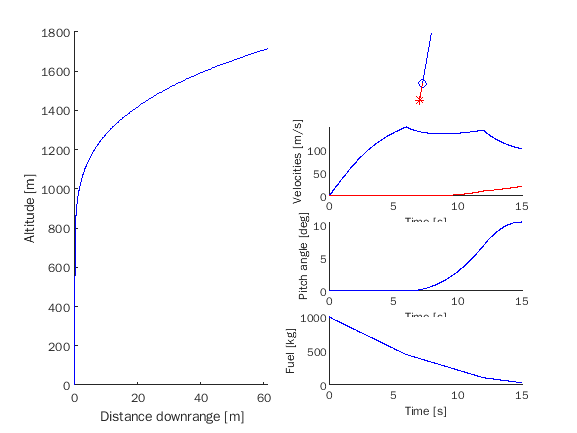
\includegraphics[width=\maxwidth{57.90265930757652em}]{figure_0.png}
\end{center}
\begin{center}
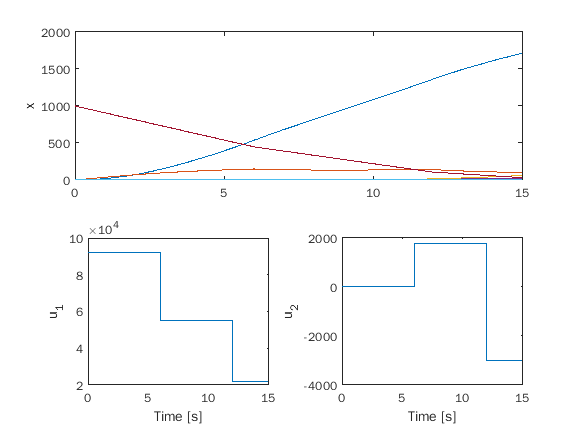
\includegraphics[width=\maxwidth{57.90265930757652em}]{figure_1.png}
\end{center}
\begin{matlabtableoutput}
{
\begin{tabular} {|c|c|c|c|c|c|c|c|}\hline
\mlcell{ } & \mlcell{altitude} & \mlcell{vel\_vert} & \mlcell{distance} & \mlcell{vel\_horiz} & \mlcell{pitch} & \mlcell{pitch\_rate} & \mlcell{fuel} \\ \hline
\mlcell{1} & \mlcell{1.7137e+03} & \mlcell{101.5699} & \mlcell{61.3932} & \mlcell{20.7220} & \mlcell{10.4151} & \mlcell{-0.0728} & \mlcell{32.2600} \\ 
\hline
\end{tabular}
}
\end{matlabtableoutput}


\begin{par}
\begin{flushleft}
\subsection*{Open Loop Control - Dynamic}
\end{flushleft}
\end{par}

\begin{par}
\begin{flushleft}
Next, a more dynamic open loop controller was attempted. This controller linearises the non-linear rocket model using Jacobians to calculate ${\textrm{Df}}_x$ and ${\textrm{Df}}_u$. Using these Jacobians, the system is linearised at each time step, substituting in the current rocket state and inputs to generate the state space matrices $\mathit{\mathbf{A}}$ and $\mathit{\mathbf{B}}$.
\end{flushleft}
\end{par}

\begin{par}
\begin{flushleft}
Using these matrices, the equation for the next required $u$ to achieve a given $x_{\textrm{target}}$ was derived from the following equations:
\end{flushleft}
\end{par}

\begin{par}
$$\dot{x} =\mathit{\mathbf{A}}\cdot x+\mathit{\mathbf{B}}\cdot \;u$$
\end{par}

\begin{par}
$$x_{\textrm{target}} =\dot{x} +x$$
\end{par}

\begin{par}
\begin{flushleft}
If we rearrange these we get the following equation for the required $u$:
\end{flushleft}
\end{par}

\begin{par}
$$u={\mathit{\mathbf{B}}}^{-1} \left(x_{\textrm{target}} -x-\mathit{\mathbf{A}}\cdot x\right)$$
\end{par}


\vspace{1em}
\begin{par}
\begin{flushleft}
Using this equation, a controller was designed to take the linearised state space system as well as a target state, and provide the required inputs to achieve that state. 
\end{flushleft}
\end{par}

\begin{par}
\begin{flushleft}
This posed the problem of requiring knowledge of how we want to system to respond, and what suitable target states are for the controller. 
\end{flushleft}
\end{par}

\begin{par}
\begin{flushleft}
Initially, the system states of the static open loop controller were utilised as the target states for this controller. This however did not function as expected, and the final state of the system varied greatly from the targeted values. To resolve this, the target states for this controller were set to be a linear interpolation between some initial values and some final target state. This was found to be very difficult to tune, most likely due to the un-invertible nature of the 'thin' $\mathit{\mathbf{B}}$ matrix requiring the use of the pseudo-inverse approximation. 
\end{flushleft}
\end{par}

\begin{par}
\begin{flushleft}
Despite this a controller was tuned to closely meets the specified requirements, and it's performance can be seen in the figures and tables below.
\end{flushleft}
\end{par}

\begin{center}
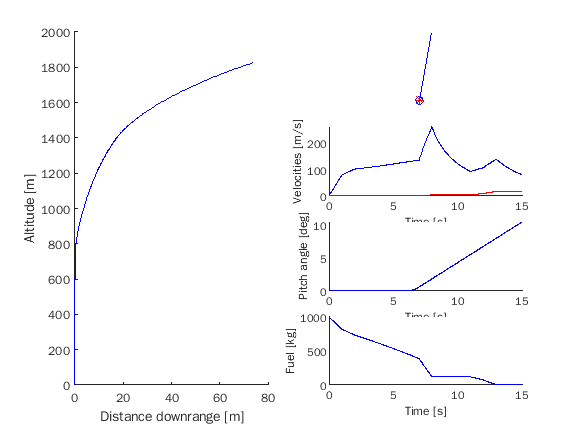
\includegraphics[width=\maxwidth{57.90265930757652em}]{figure_2.png}
\end{center}
\begin{center}
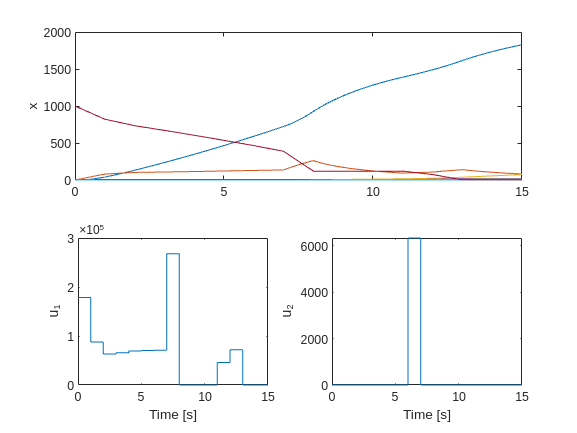
\includegraphics[width=\maxwidth{57.90265930757652em}]{figure_3.png}
\end{center}
\begin{matlabtableoutput}
{
\begin{tabular} {|c|c|c|c|c|c|c|c|}\hline
\mlcell{ } & \mlcell{altitude} & \mlcell{vel\_vert} & \mlcell{distance} & \mlcell{vel\_horiz} & \mlcell{pitch} & \mlcell{pitch\_rate} & \mlcell{fuel} \\ \hline
\mlcell{1} & \mlcell{1.8267e+03} & \mlcell{80.4996} & \mlcell{74.0839} & \mlcell{18.3334} & \mlcell{10.5192} & \mlcell{1.2383} & \mlcell{2.1439} \\ 
\hline
\end{tabular}
}
\end{matlabtableoutput}


\begin{par}
\begin{flushleft}
\subsection*{Closed Loop Controller}
\end{flushleft}
\end{par}

\begin{par}
\begin{flushleft}
The final attempted controller for this system is a closed loop gain controller via pole placement. This form of controller also required the linearisation of the system model, and utilised the same Jacobains from the previous controller to produce the $\mathit{\mathbf{A}}$ and $\mathit{\mathbf{B}}$ matrices.
\end{flushleft}
\end{par}

\begin{par}
\begin{flushleft}
Once the poles are placed, the controller gains will be used to close the loop with the following equation:
\end{flushleft}
\end{par}

\begin{par}
$$u=-\mathit{\mathbf{K}}\left(x-x_{\textrm{target}} \right)$$
\end{par}

\begin{par}
\begin{flushleft}
The first challenge with this controller design was the placement of the system poles. As this system is not time invariant, the optimal pole locations and thereby controller gains are not constant. Due to this, the use of the matlab \texttt{'place()'} command was not feasible, as the optimal locations for all system poles at each given time-step would be very tedious to calculate. 
\end{flushleft}
\end{par}

\begin{par}
\begin{flushleft}
To overcome this, a static linear quadratic regulator was used to calculate the controller gains at each time step. This controller required inputs $\mathit{\mathbf{A}}$ and $\mathit{\mathbf{B}}$ (the linearised system model) as well as $\mathit{\mathbf{Q}}$ and $\mathit{\mathbf{R}}$. Both the $\mathit{\mathbf{Q}}$ and $\mathit{\mathbf{R}}$ matrices sets bounds on the controller, specifying how much we wish the controller to be able to deviate from our target value, with larger values allowing for larger deviation.
\end{flushleft}
\end{par}

\begin{par}
\begin{flushleft}
To tune this controller, the selection of input and output bounds must be completed, as well as the selection of the target states for the controller to achieve. Due to the large number of variables to tune for this controller, it was decided that the system state matrix saved from the first controller would be used for the target values, to decrease the number of parameters. From here the bounds were tuned on a basis of which final states were deemed to be most important for the controller to achieve. In the case of this controller, emphasis was placed on both the pitch angle and pitch rate of the rocket, allowing for more deviation in the final state of the fuel. 
\end{flushleft}
\end{par}

\begin{par}
\begin{flushleft}
The final tuned controller can be seen operating below. Due to the emphasis placed achieving the pitch angle and rate, it can be seen that the controller maintains this value. It can also be seen from that table below that the controller closely meets the majority of requirements outlined.
\end{flushleft}
\end{par}

\begin{center}
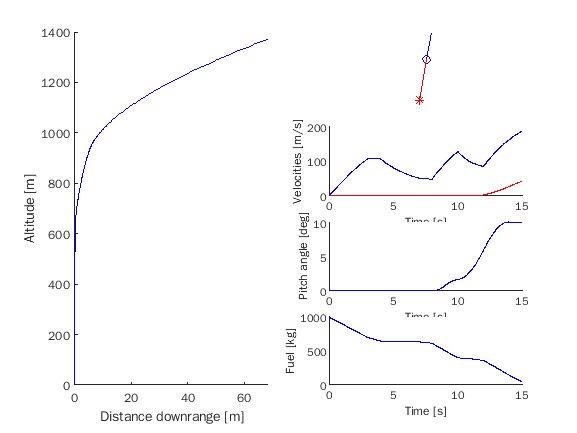
\includegraphics[width=\maxwidth{57.90265930757652em}]{figure_4.png}
\end{center}
\begin{center}
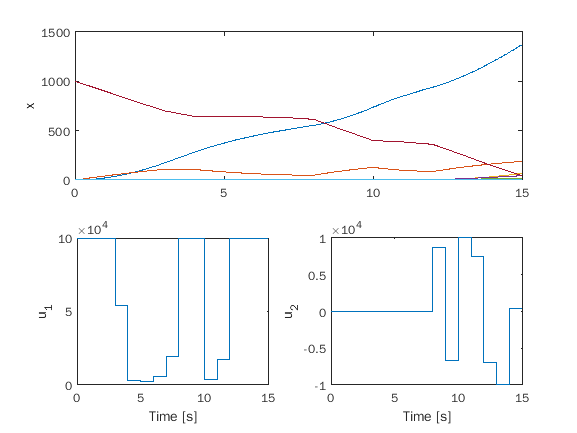
\includegraphics[width=\maxwidth{57.90265930757652em}]{figure_5.png}
\end{center}

\begin{matlabtableoutput}
{
\begin{tabular} {|c|c|c|c|c|c|c|c|}\hline
\mlcell{ } & \mlcell{altitude} & \mlcell{vel\_vert} & \mlcell{distance} & \mlcell{vel\_horiz} & \mlcell{pitch} & \mlcell{pitch\_rate} & \mlcell{fuel} \\ \hline
\mlcell{1} & \mlcell{1.3722e+03} & \mlcell{188.2942} & \mlcell{68.4396} & \mlcell{43.4865} & \mlcell{10.1215} & \mlcell{-0.0023} & \mlcell{43.9700} \\ 
\hline
\end{tabular}
}
\end{matlabtableoutput}

\section*{Conclusions}

\begin{par}
\begin{flushleft}
Both open loop and closed loop controllers have been designed to meet the outlined specifications for this system. 
\end{flushleft}
\end{par}

\begin{par}
\begin{flushleft}
It can clearly be seen from the system plots above that the initial open loop controllers provides the best response in regard to both the final state of the system, and the path taken. This controller however implements no form of feedback, and as such has no method of correcting for external perseverances.
\end{flushleft}
\end{par}

\begin{par}
\begin{flushleft}
Although both the dynamic open loop and closed loop controllers achieved the majority of system requirements, the tuning of the controllers was complex and tedious. However, the closed loop controller integrates feedback into the system and may allow for the rejection/correction of external errors. 
\end{flushleft}
\end{par}

\begin{par}
\begin{flushleft}
Overall, of the three controllers designed and discussed, the static open loop controller provides the best response and easiest implementation for a system with no external forces, while the closed loop controller provides a more robust controller design.
\end{flushleft}
\end{par}

\end{preview}
\end{document}
